\documentclass[a4j,12pt]{ujarticle}

\usepackage{amsmath,amssymb}
\usepackage{enumerate,bm}
\usepackage[dvipdfmx]{graphicx}
\usepackage[dvipdfmx]{pict2e}
%\usepackage[dvipdfmx,colorlinks=faluse,citecolor=black,urlcolor=blue]{hyperref}%
\usepackage{url}
\usepackage{ketpic,ketlayer}
\usepackage{wrapfig}

\newcommand{\bs}{$\backslash$}
\newcommand{\br}[1]{\{#1\}}
\setcounter{figure}{0}

\newcommand{\figcap}[1]{
\addtocounter{figure}{1}図\thefigure.\ #1}

\newcommand{\dint}{\displaystyle\int}
\newcommand{\dlim}{\displaystyle\lim}

\newcounter{Li}
\newcounter{Lii}
\newcounter{Liii}

\topmargin =-0.8cm 
\oddsidemargin =0.1cm
\textheight=23.5cm
\textwidth=15.7cm


\newcommand{\chosha}[5][11zw]{%
\noindent
\hspace*{#1}\Ltab{#2}{#3}#4\\
\hfill #5
}

\renewcommand{\refname}{参考文献}

\begin{document}

\begin{center}

{\bf \Large KeTMath による課題送受・採点処理・結果分析}

\end{center}

\mbox{}

\begin{center}

KeTCindyセンター 高遠 節夫

Setsuo Takato, KeTCindy Center, Magnolia Inc.


長野高専・一般科 濱口 直樹

Naoki Hamaguchi, National Institute of Technology (KOSEN), Nagano College

山口大学・教育学部 北本 卓也

Takuya Kitamoto, Faculty of Education, Yamaguchi University

\end{center}

\section{KeTCindyとKeTCindyJS}

Cinderellaは,1993年から1999年にかけて,J.Richter-Gebert氏とU.H.Kortenkamp氏によって開発された動的幾何である(\cite{Cinderella1}).さらに,両氏はCinderellaに3D機能やプログラム言語CindyScriptを組み込んだCinderella.2(以下Cindy)をリリースした(\cite{Cinderella2}).
CindyScriptは通常の言語に近く,数値や文字列のデータおよびファイル操作が可能である.一方,著者(高遠)のグループは,2006年以来,図のデータからMaple, Mathematica, Scilab, Rにより\TeX の描画コードTpic を書き出して,\TeX 文書の図作成に利用するためのマクロ集\ketpic を開発してきた.この\ketpic の対話性をより高めるために,著者らは2014年にKortenkamp氏を招聘してジョイントワークショップを開き,その成果として\ketcindy の最初の
バージョン1.0ができあがった.\ketcindy は以下の流れで\TeX の図を作成する.\vspace{-2mm}

\begin{enumerate}
\item \ketcindy の雛形ファイルをクリックして,Cindyを立ち上げる\\
・\ketcindy のマクロライブラリ読み込みと実行ボタンの配置が実行される.\\
・なお最近のCindyでは,Kortenkamp氏に依頼して\ketcindy で用いられる\\
 Java関数群を最初から\verb|KetCindyPlugin.jar|として組み込んでもらっている.\vspace{-2mm}
\item Cindyの幾何要素(点など)と\ketcindy の描画関数から画面上に図を作成する.\\
・画面の図を見ながら,幾何要素と描画関数の引数などを変更することができる.\\
・同時に描画コード作成のためのRコマンドリスト(\verb|GLIST|)が作成される.

\vspace{-2mm}
\item 画面上の\verb|Figure|(描画ファイル作成ボタン)をクリックするとRが呼び出される.\\
・まず,(3)の\verb|GCLIST|により描画コードから成る\TeX ファイルが作成される.\\
・次に\TeX を起動して,確認用の\TeX ファイルをコンパイル,PDFを作成する.\\
  注:図ファイルは\verb|\input|でメインファイルに挿入される.\vspace{-1mm}
\end{enumerate}

\ketcindy からは,RだけでなくMaximaやgccを呼び出すこともできる.gccは\ketcindy 曲面描画の隠線処理を高速化するためのものである.また,Maximaの数式処理計算の呼び出しは,例えば次のように行われる.\vspace{-1mm}

\begin{itemize}
\item 単独関数の呼び出し\\
 \verb|Mxfun("1","integrate",["x^2","x",0,1]);|\\
  注:\verb|Mxfun("1","integrate("x^2,x,0,1",[]);|でもよい.\vspace{-2mm}
\item 関数群の呼び出し\footnote{後述のKeT-LMSで実際に用いられる}\\
 \verb|cmdL=[|\\
 \verb|  "i1:x^2-4*x",[],|\\
 \verb|  "i2:(1)/(x)+sin(x)",[],|\\
 \verb|  "o1:integrate([i1,i2],x)",[],|\\
 \verb|  "o1[1]::o[2]",[]|\\
 \verb|];|\\
 \verb|CalcbyM("ans",cmdL,[]|\\
・実行は,上記コマンドをScriptEditorに記述して\verb|Figure|を押すだけでよい.\\
・結果は\verb|ans=[1/3*x^3-2*x,log(x)-cos(x)]"|となる.\vspace{-1mm}
\end{itemize}

2016年,ミュンヘン工科大学のGebert研究室グループは,Cindyとほぼ互換なHTMLコンテンツを作成するフレームワークCindyJSを開発した\footnote{「CindyJS」で検索すると URL https://cindyjs.orgが見つけられる}.これに対応して,CindyにもCindyJSのHTMLを書き出す機能が追加された.そこで,著者らは\ketcindy で定義されている関数を組み込んだHTMLを作成する機能\ketcindy JSを\ketcindy に追加した.\ketcindy の組み込みの手順は以下の通りである.\vspace{-2mm}

\begin{enumerate}
\item Cindyファイル(例えばsample.cdyとする)のトップメニューにある「HTMLに書き出す」を選択してCindyJSのHTMLファイルsample.htmlを出力する.\vspace{-2mm}
\item KeTJSのボタンを押すと,1に\ketcindy を組み込んだHTMLが作成される\footnote{OnはホームページからCindy.jsを,OffはローカルフォルダからCindy.jsを読み込む}.\vspace{-1mm}
\end{enumerate}

上記の2を実行するプログラムについて少し説明を加える.まず,Cindyが出力するファイルsample.htmlを
1行ずつ読み込む.そのためには,\ketcindy に追加されている関数\verb|Readlines|が用いられる.\\
\hspace*{2zw}\verb|Lines=Readlines(Dircdy,sample.html);|\\
ここで,DircdyはCindyファイルのパスを表すグローバル変数で,やはり\ketcindy で定義されている.
次に,\ketcindy のライブラリをsample.htmlのInitializationスロット\footnote{Cindyではプログラムの単位をスロットといい,initializationは初期設定の場合のみ実行される.}
に追加する.ただし,ライブラリの総行数は20000行を超えるので,ファイルサイズを抑えるために次の工夫を施している.\vspace{-1mm}
\begin{itemize}
\item  \ketcindy のライブラリで定義されているすべての関数について\\
\hspace*{2zw}関数名,先頭行,最終行,内部で使われている\ketcindy 関数群\\
のリストをライブラリの更新ごとに作成する.\vspace{-2mm}
\item sample.htmlのdraw, initializationスロットで使われている関数を再帰的に拾い出して,
その関数の定義だけをinitializationスロットに追加する.\vspace{-1mm}
\end{itemize}

この方法により,総行数を3000行から5000行程度に抑えることを可能にした.また,sample.htmlのファイルサイズはCindyJSとKaTeXのライブラリを除き,ほとんどの場合100KB以下とかなり小さくなっている.
「ketcindy samples」で検索されるサイト\footnote{https://s-takato.github.io/ketcindysample/}には多くの\ketcindy JSのサンプルが掲載されている.

\section{KeTMathの開発とkettaskによる問題の配付}

2020年度はコロナ流行のため,多くの教育機関でオンライン授業の利用など,従来の授業方式の変更を余儀なくされた.著者の1人(高遠)が数学を担当している短期大学校でも,授業開始が6月に延期された上に,対面方式にせよ接触をできるだけ避ける工夫が必要となった.講義については,東邦大に所属するときからずっと\TeX で作成したスライドを使用していた\footnote{スライドには適宜\ketcindy で作成したフリップアニメーションを挿入している.}ので,オンラインでも,双方向性を保ち授業の流れが単調にならないように工夫することで容易に対応できたが,課題のやりとりでは数式をどうするかが大きな問題になった.そこで,1次元の簡易数式ルールを作り,そのルールに従って記述された数式を即時に2次元\TeX 数式に変換して表示するHTMLアプリKeTMathを\ketcindy JSで開発した\footnote{「ketcindy samples」の他に「ketcindy home」にアクセスしてそのまま利用することができる.}.例えば,
分数$\dfrac{a}{b}$,平方根$\sqrt{x}$は,KeTMathルールではそれぞれfr(a,b),\ sq(x)と記述すればよい.KeTMmathの初期バージョンでは,PCやスマホのキーボードを用いてKeTMath数式を入力すようにしていたが,スマホのキーボードは種類が多いために,特殊記号を誤って入力してしまうという欠点があった.そこで,KeTMathの画面上にキーボードを配置するようにした.

\begin{center}
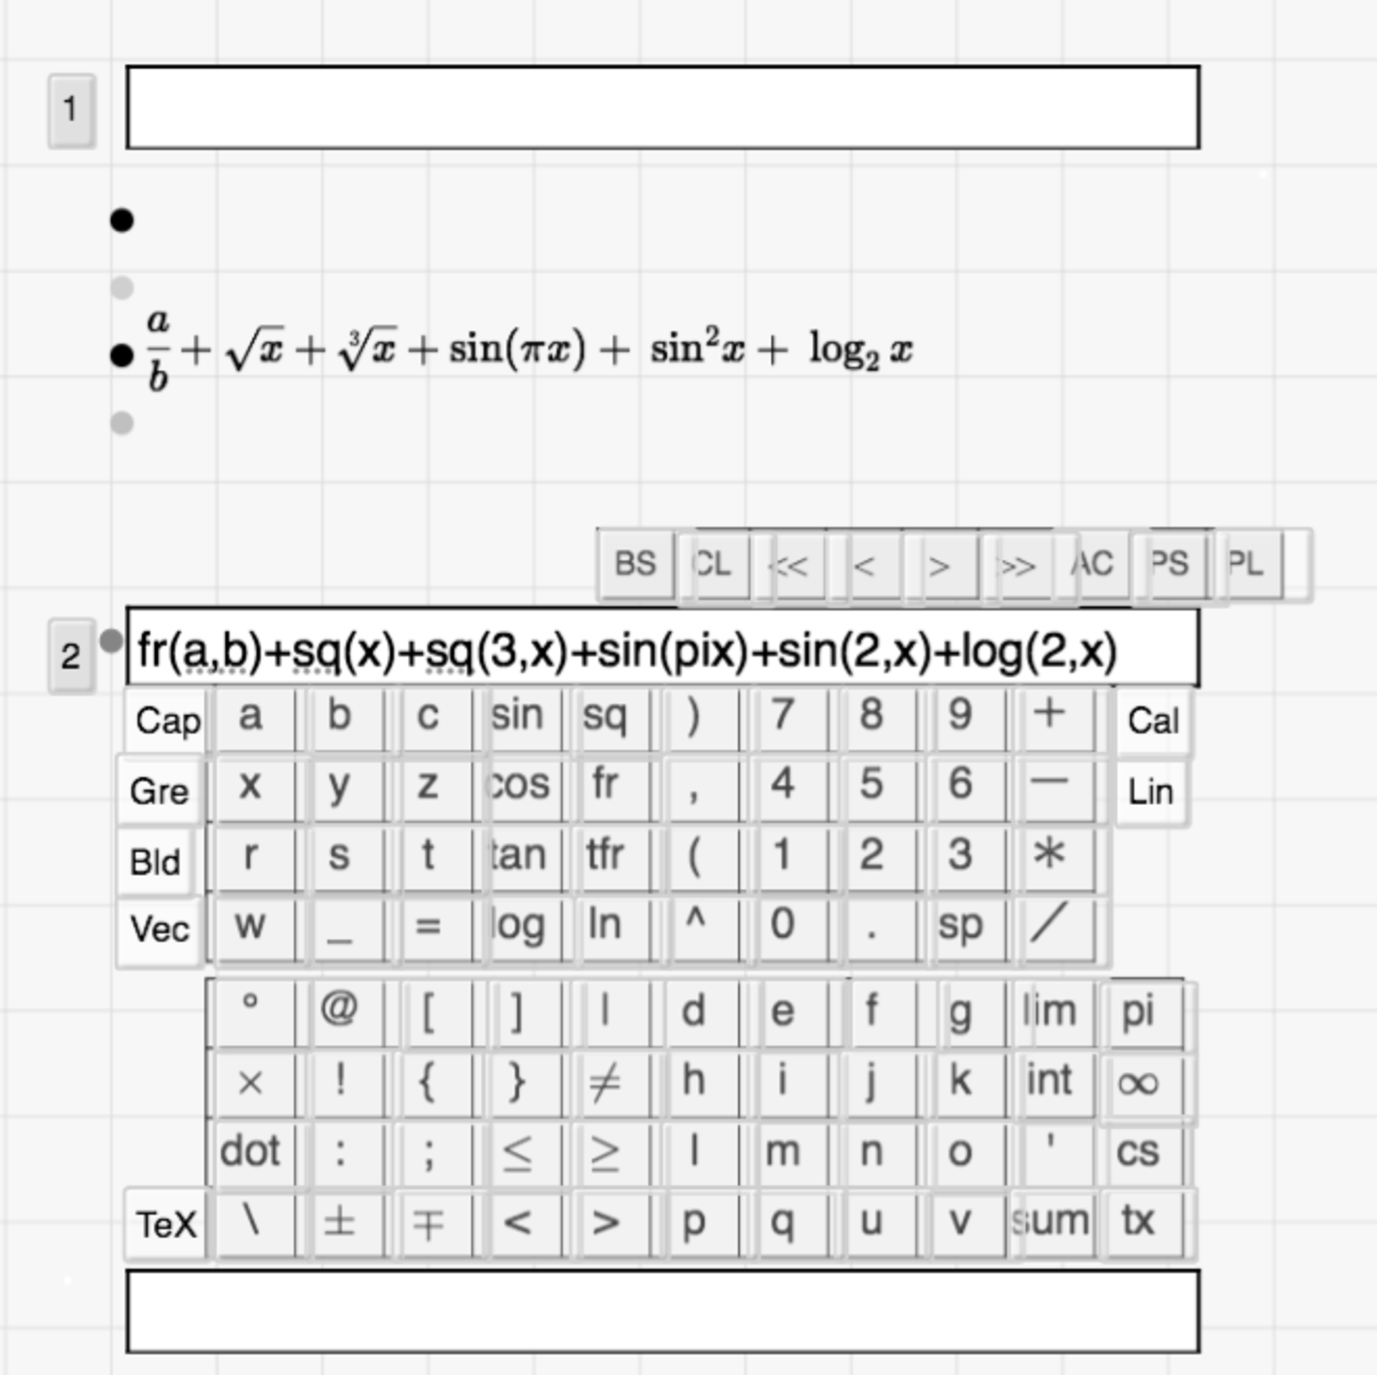
\includegraphics[bb=0.00 0.00 661.00 660.00,height=90mm]{fig/ketmathbw.pdf}\hspace{5mm}
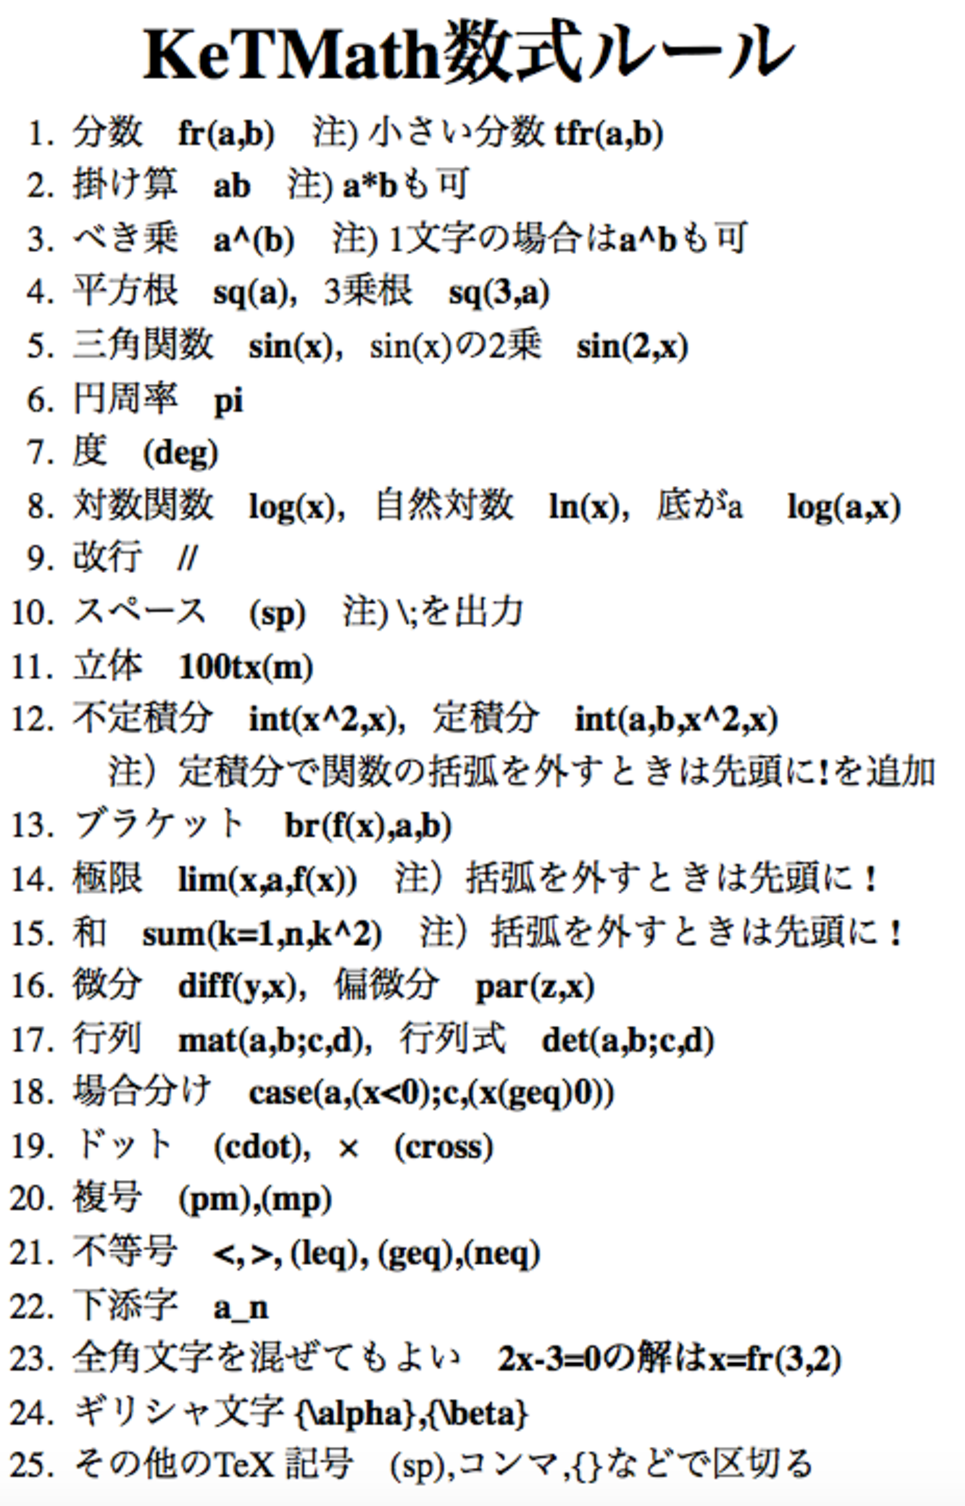
\includegraphics[bb=0.00 0.00 463.00 723.00,height=90mm]{fig/ketmathrule.pdf}\\
\addtocounter{figure}{1}Fig.\thefigure\ \ KeTMathの画面とKeTMathルール\vspace{-1mm}
\end{center}

KeTMathのプログラミングでは文字列の解析が重要である.Cindyの持つ関数\\
\hspace*{2zw}length(長さ), substring(部分列), tokenize(分割), indexof(検索), %
replace(置換)\\
に加えて,KeTMath数式を解析するための関数\\
\hspace*{2zw}\Ltab{60mm}{Bracket(文字列,"()")}括弧の位置とレベルを返す\\
\hspace*{2zw}\Ltab{60mm}{Getlevel(文字列,",","()"}括弧についてのコンマの位置とレベルを返す\\
などをketcindyに組み込んでいる.

また,KeTMath数式をCindy形式に変換するTocindyform,Maxima形式に変換するTomaxformも追加した.これらの関数を用いれば,1つのKeTMath数式から,\TeX だけでなくグラフを描くための関数形式やMaximaで数式計算するための関数形式を出力することもできる.\\
\hspace*{4zw}Totexform("fr(1,x)") $\Longrightarrow$\verb|\frac{1}{x}|\\
\hspace*{4zw}Tocindyform("fr(1,x)")  $\Longrightarrow$ \verb|(1)/(x)|\\
\hspace*{4zw}Tomaxform("fr(1,x)")  $\Longrightarrow$ \verb|(1)/(x)|

\vspace{1mm}

\noindent
「高専・大学 数学・大日本図書」で検索される大日本図書の教科書ページ\\%
\hspace*{2zw}\verb|https://www.dainippon-tosho.co.jp/college_math/|\\
には上記の関数を利用して作成したWeb Contentsが掲載されている.


\begin{center}
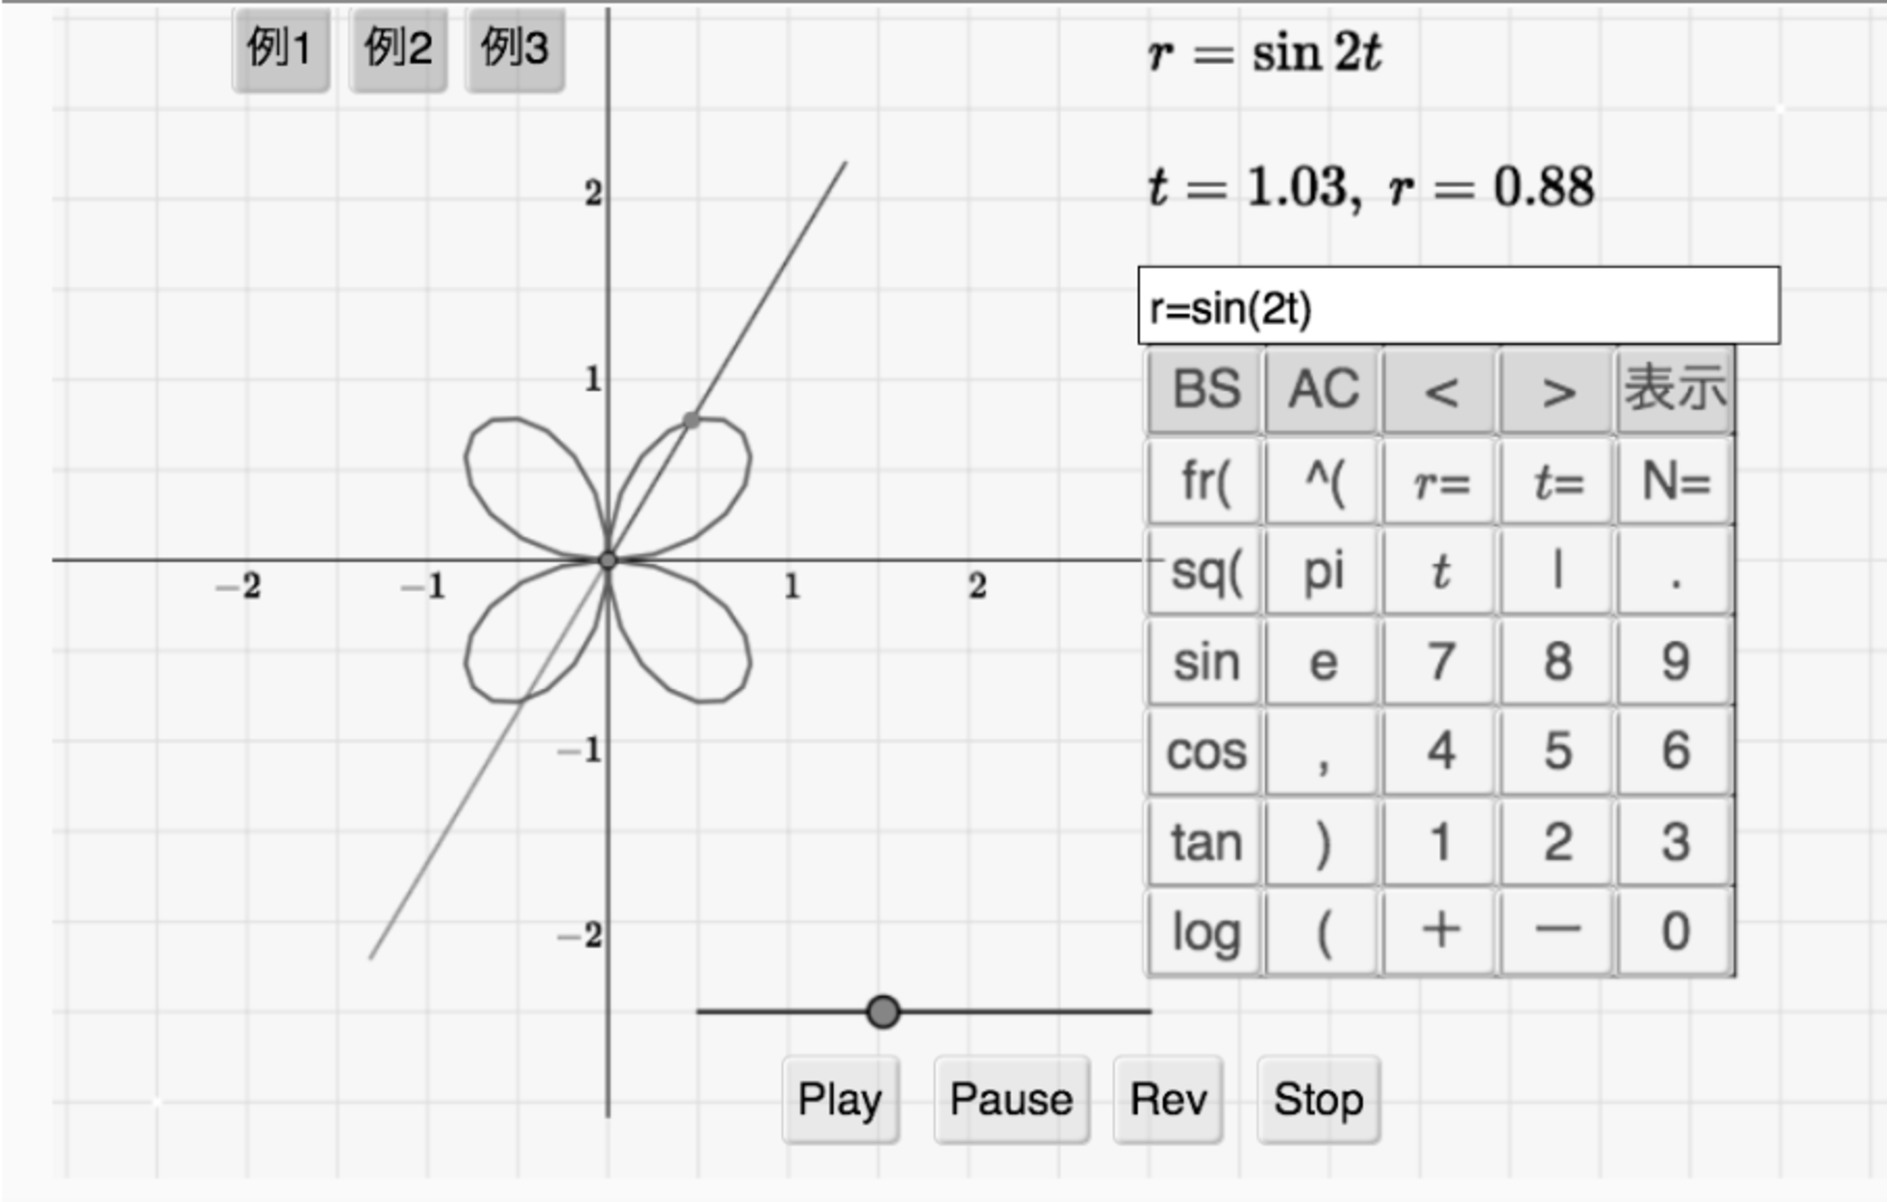
\includegraphics[bb=0.00 0.00 906.00 577.00,height=45mm]{fig/dntcalbw.pdf}
%
\hspace{5mm}%
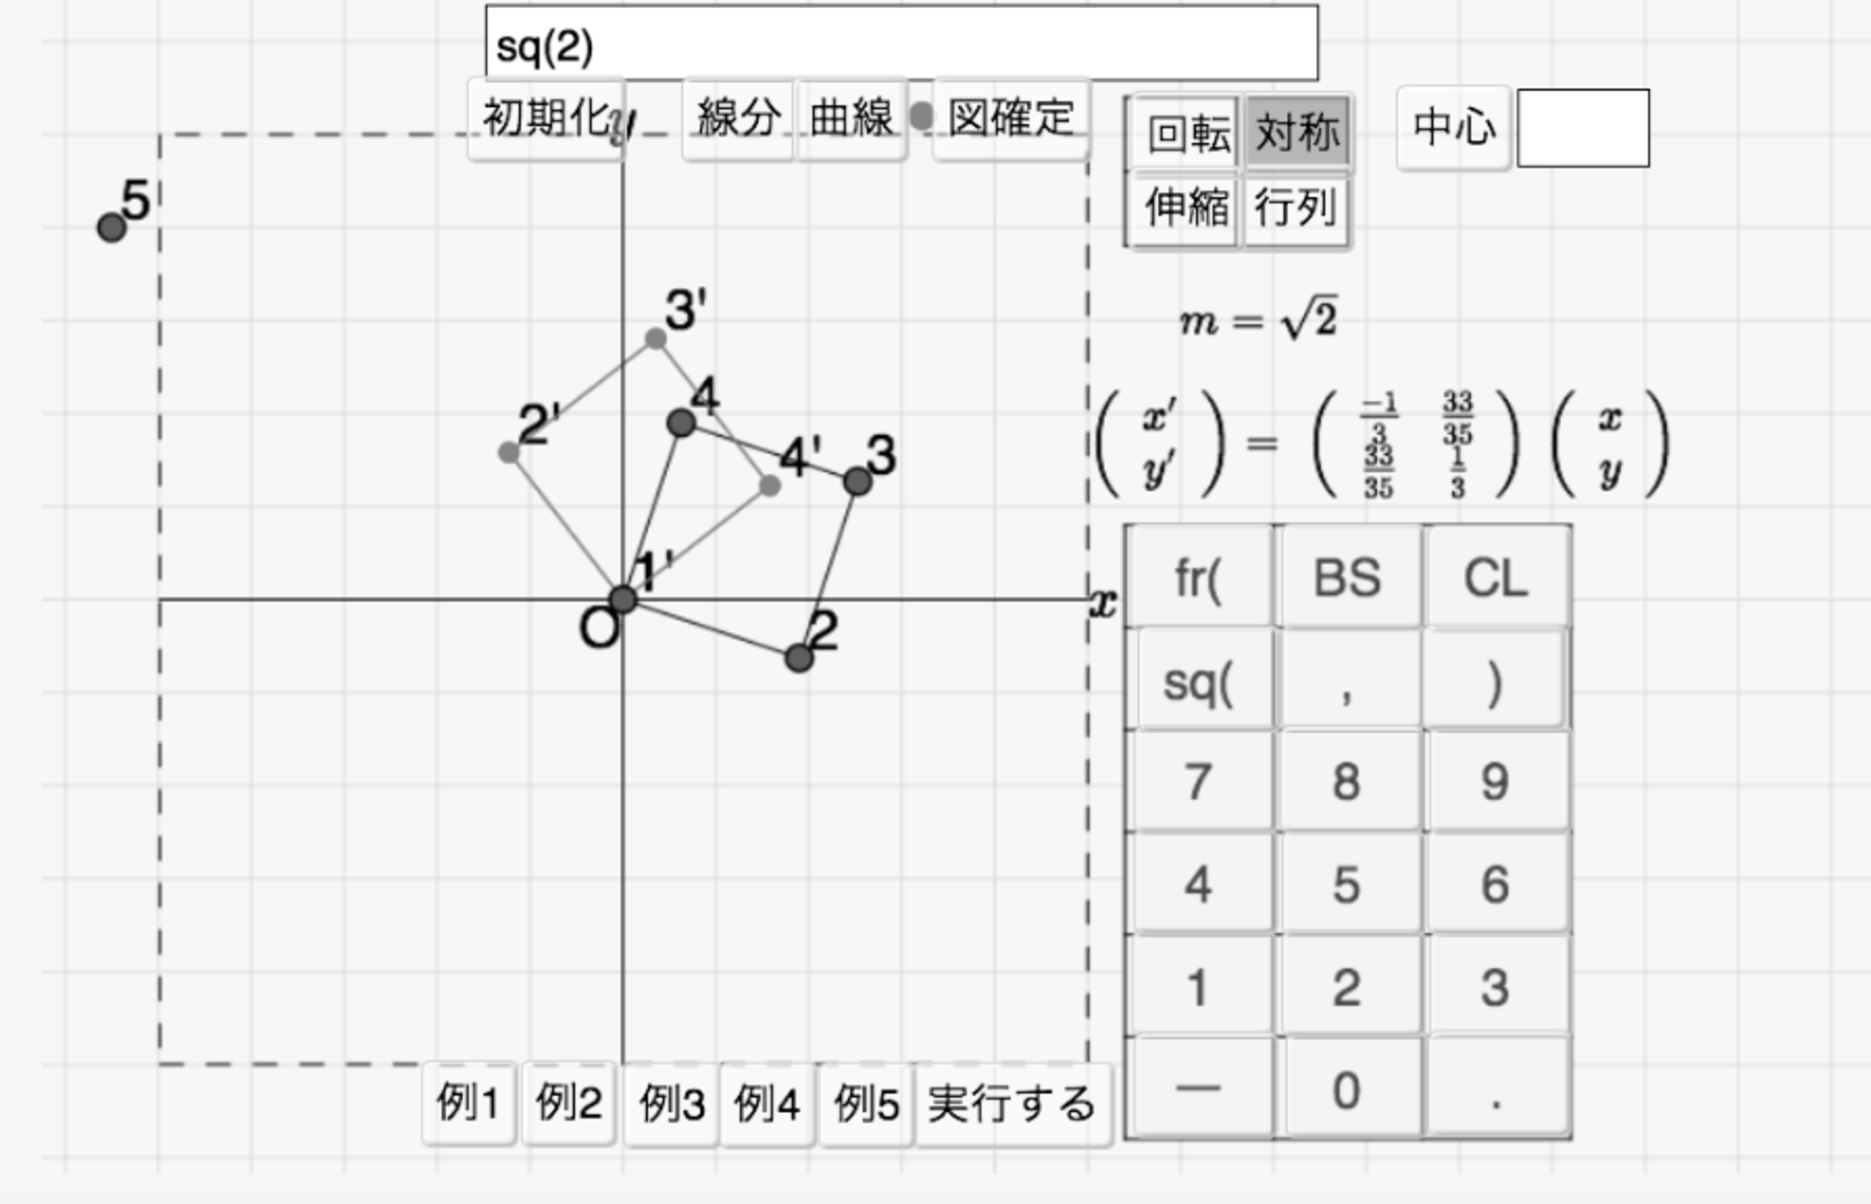
\includegraphics[bb=0.00 0.00 898.00 578.00,height=45mm]{fig/dntlinbw.pdf}

\addtocounter{figure}{1}Fig.\thefigure\ \ インタラクティブなWeb教材例\vspace{-1mm}

\end{center}

通常の授業では,課題のやり取りはプリントで行われる.これに対して,
KeTMathを単体で用いたときは次のようになる.\vspace{-1mm}
\begin{enumerate}
\item 学生が課題の書かれたPDFを見られるようにする.このPDFは講義スライドでもいいし,独立に作成してもよい.\vspace{-2mm}
\item 学生はその課題をノートなどで解いて,解答をKeTMathルールで作り,
KeTMathで確認してから教員にメールなどで送信する.\vspace{-2mm}
\item 教員は回収した解答をKeTMathにコピー&ペーストして確認しながら採点する.\vspace{-1mm}
\end{enumerate}

しかし,かなりの数の学生はKeTMathで確認することをせずに間違った数式をそのまま送ってきたり,√2などと特殊文字を使ったりしていた.そこで,問題自体を組み込んだ出題アプリKeTTaskを作成して配付することにした.
同時に,教員が採点するためののアプリKeTscoreも作成することにして,
それぞれの雛形ファイルから問題ごとのファイルを生成する\ketcindy のプログラムtoolketmath.cdyを開発した.また,問題の配付と回収はオンライン学習システム(以下OLS)の1つであるGoogle Classroom(以下GC)を利用することにした\footnote{個人ベースだったのでGCを用いたが,TeamsやMoodleなどでも同様である.}.まず,課題の配付については次のようにする.\vspace{-1mm}
\begin{enumerate}
\item 1つのフォルダにkettaskorg.html, ketscoreorg.html, toolketmath.cdy\footnote{\ketcindy のライブリを使うため,「ketcindy home」からダウンロードしてインストールしておく.}とCindyJSとKaTeXのライブラリフォルダketcindyjsを入れて,フォルダdataを作成する.\vspace{-2mm}
\item dataの中に学生リスト(student2022.txtなど)とKeTMathルールをベースとした文法に従ってKeTMathルールで記述された問題ファイル(question1130-01.txtなど)を入れる.\\
\begin{minipage}[t]{68mm}
\begin{center}
学生リスト
\end{center}
\hspace*{2zw}01AA\\
\hspace*{2zw}02BB\\
\hspace*{2zw}03CC\\
\hfill{\small 注)番号+イニシャルなどの識別名}
\end{minipage}\hspace{6mm}%
\begin{minipage}[t]{68mm}
\begin{center}
問題ファイル
\end{center}
\hspace*{2zw}Q\hfill{\small 注)ファイル名から番号追加}\\
\hspace*{2zw}次の関数を微分せよ\\
\hspace*{2zw}$[1]$ y=x\^{}4-3x\^{}3+x\^{}2+2x-3\\
\hspace*{2zw}$[2]$ y=e{}\^{}x+log(x)\\
\hspace*{2zw}Sheet\hfill{\small 注)解答欄}\\
\hspace*{2zw}$[1]$ y'=  ::5\hfill{\small 注)配点}\\
\hspace*{2zw}$[2]$ y'=  ::5\\
\hspace*{2zw}Ans\hfill{\small 注)正解}\\
\hspace*{2zw}$[1]$ 4x\^{}3-9x\^{}2+2x+2\\
\hspace*{2zw}$[2]$ e{}\^{}x+fr(1,x)\\
\end{minipage}\vspace{-1mm}

\item toolketmath.cdyを立ち上げ,「tasklineを作成」と「kettaskに組み込み」の
ボタンを押すと,問題,解答欄,学生データを組み込んだkettask1130-01.html(以下kettask.html)ができる.\vspace{-2mm}
\item kettask.htmlファイルを教員が用いているホスティング\footnote{著者らはgithubのPagesを利用している.}にアップして,リンク先のURLを取得する.\vspace{-2mm}
\item 4のURLをOLSのテキストをやり取りする機能\footnote{GC, Teams, Moodleではそれぞれ
「質問」「クイズ」「アンケート」} を用いて学生に配付する.\vspace{-2mm}
\item 学生はスマホなどでketask.htmlを立ち上げて,番号を入力確認してからKeTMathルールで解答を入力する.\vspace{-2mm}
\item 解答が終わったら,Recボタンを押して最下段にある記録欄に表示される解答(1行のテキストである)をOLSの回答にコピー&ペーストして送信する.なお,解答の先頭には学生番号と提出日時のデータが追加される.\vspace{-1mm}
\end{enumerate}

\begin{center}
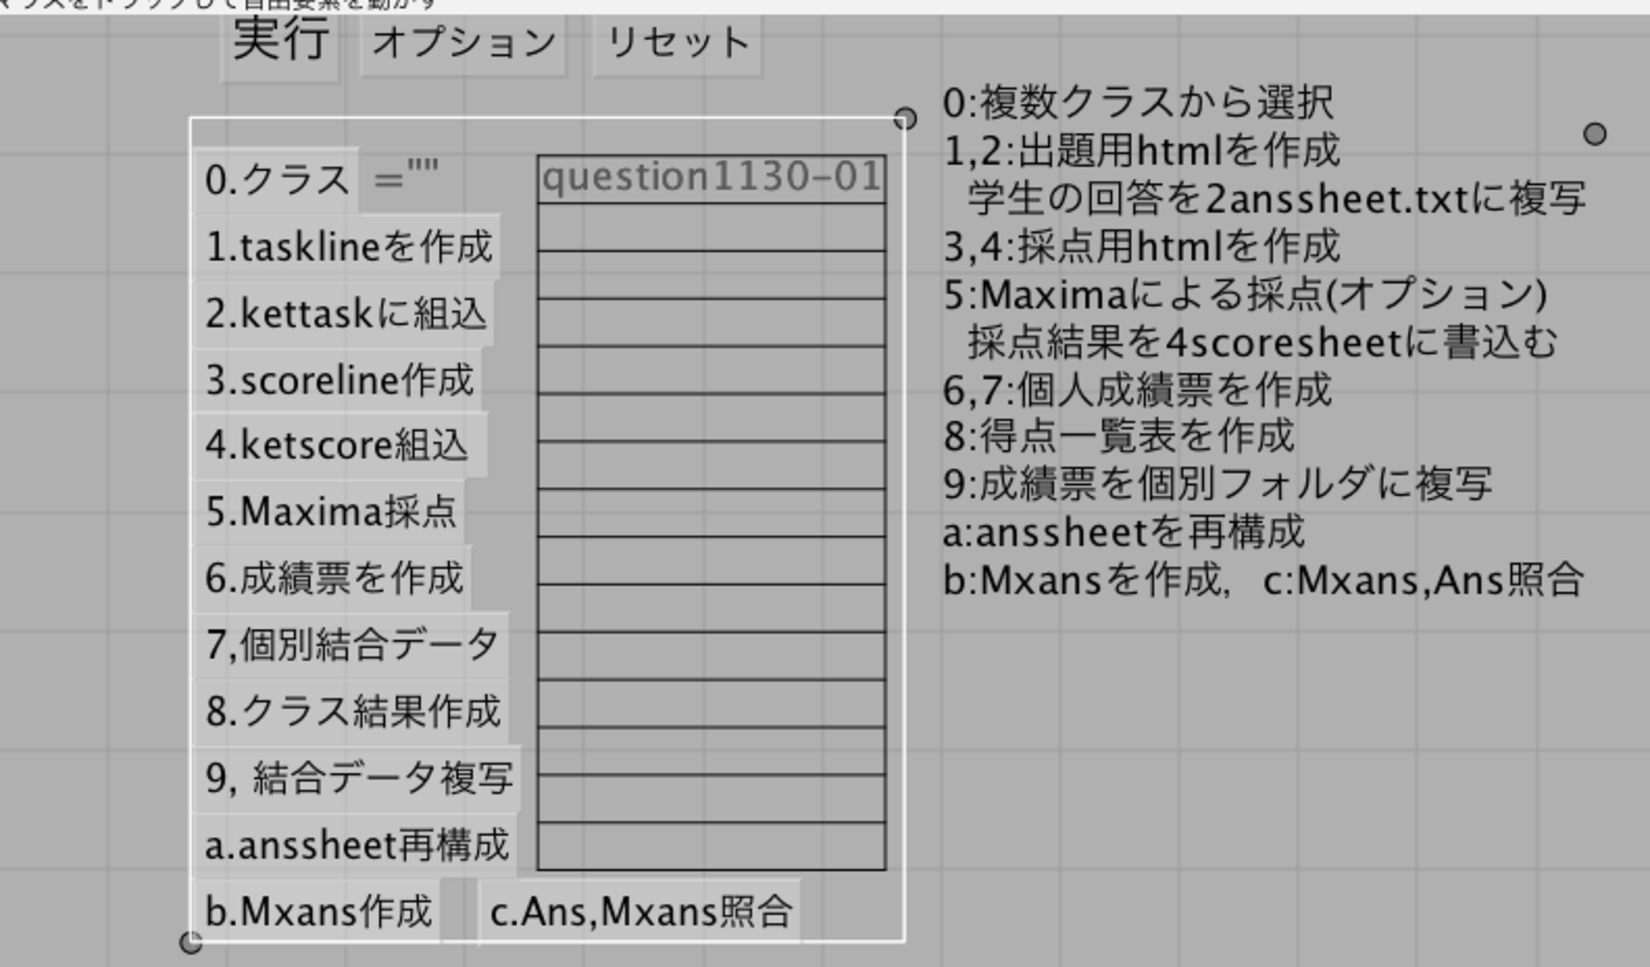
\includegraphics[bb=0.00 0.00 792.00 464.00,height=52mm]{fig/toolketmathbw.pdf}
\hspace{5mm}%
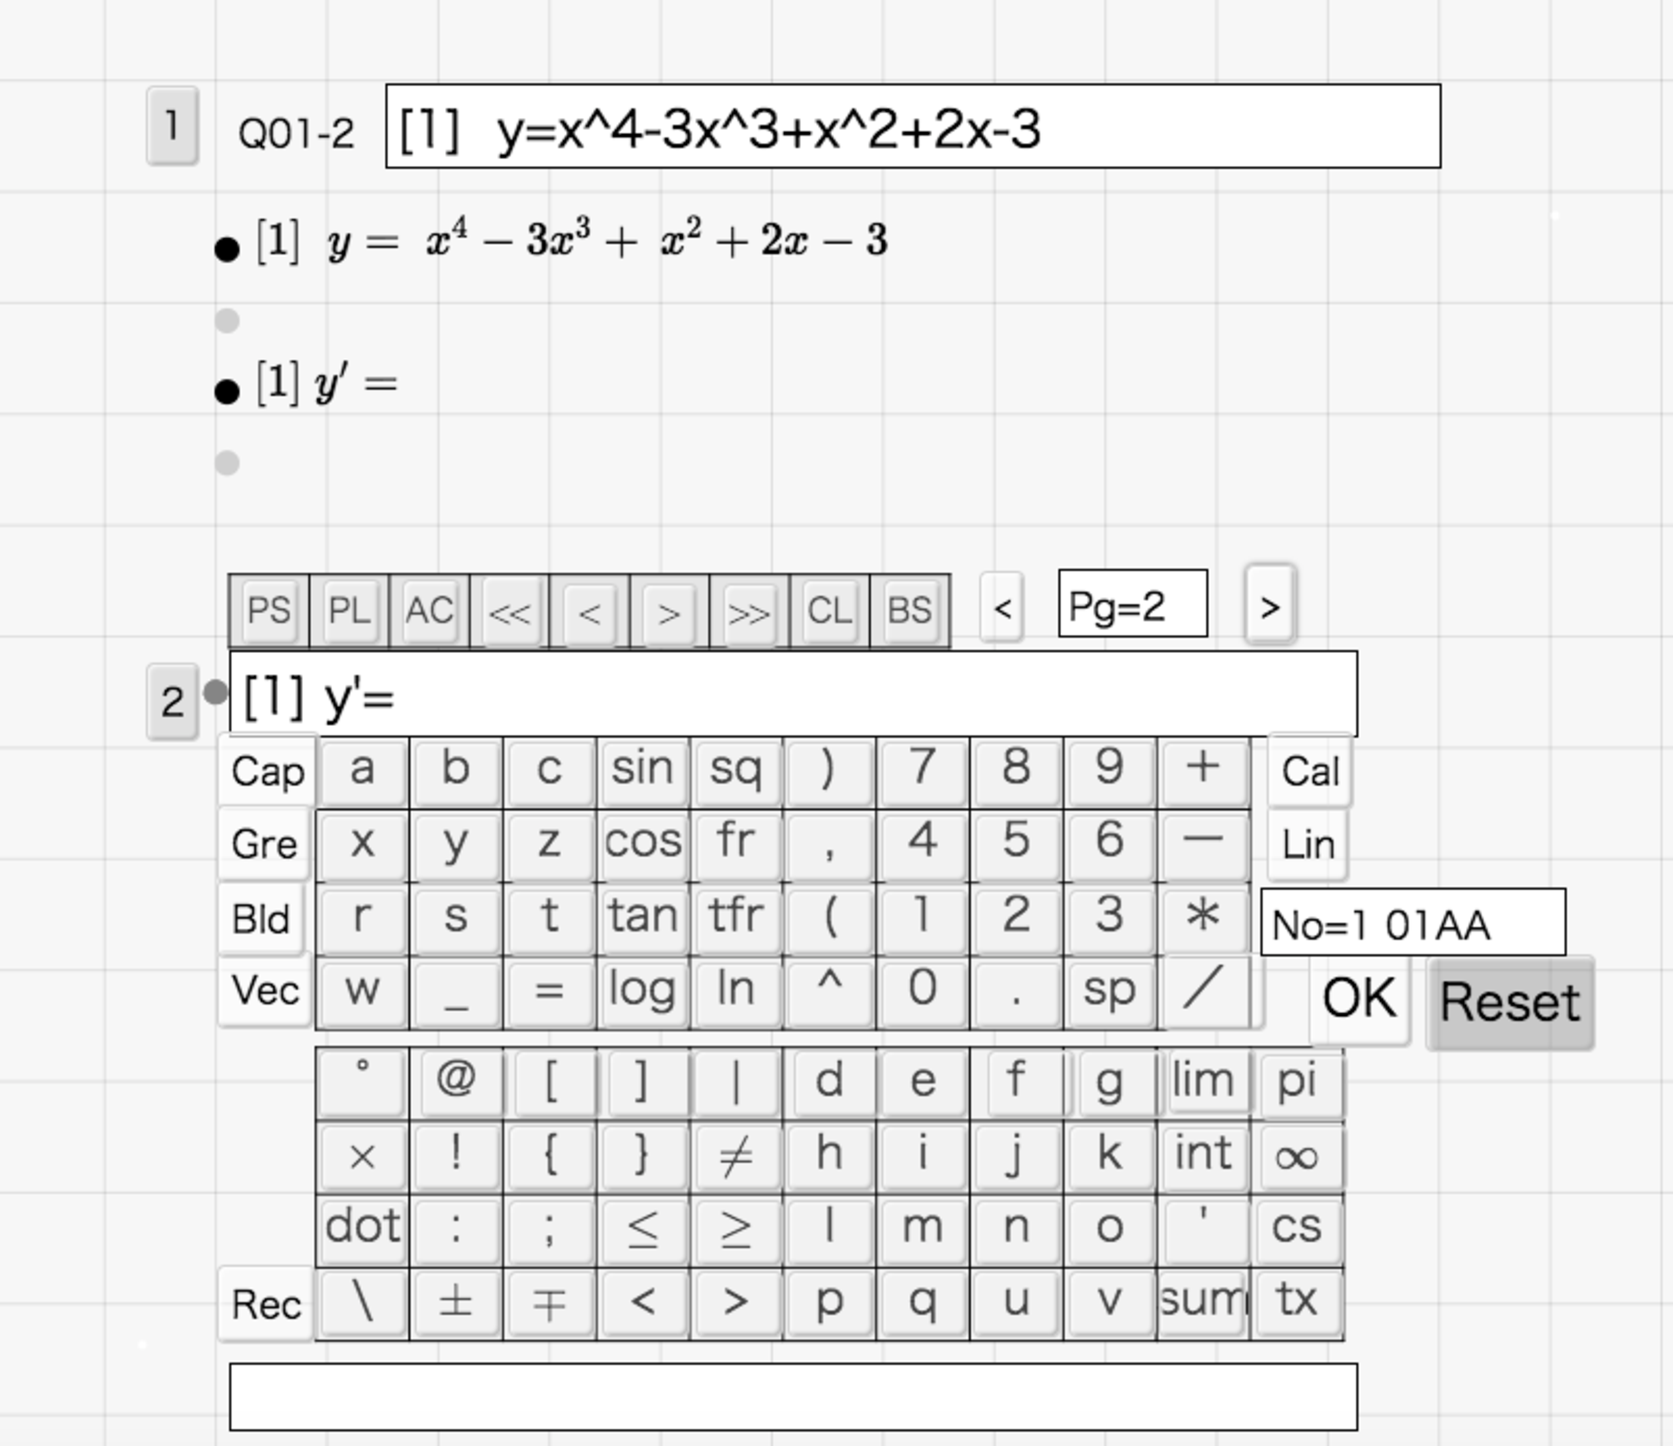
\includegraphics[bb=0.00 0.00 803.00 694.00,height=52mm]{fig/kettaskbw.pdf}
\addtocounter{figure}{1}Fig.\thefigure\ \ toolketmathallとkettaskの画面\vspace{-1mm}
\end{center}

\section{ketscoreによる採点}

学生からの回答は,OLSによって方法は多少異なるが,いずれを用いてもテキストの扱いは共通であり,1つのテキストファイル2anssheet1130-01.txt\footnote{このファイルはtoolketmathで「tasklineを作成」を実行したときに準備される.}に容易にまとめることができる .次に,oolketmath.cdyを立ち上げて,「scorelineを作成」と「ketscoreに組み込み」のボタンを押すと,問題,正解,配点,学生のデータを組み込んだ採点用のketscore.htmlができる.ketscore.htmlでは学生と問題がマトリックス形に配置されているので,学生ごとまたは問題ごとに採点することができる.画面の上段には正解,中段には学生の解答,下段には問題が表示され,それを見ながら中段の::の後に点数をつけていく.採点が終わったらRecボタンを押すと,下段にすべての解答が1行のテキストとして表示されるので,これを確定データのためのファイル4scoresheet.txt\footnote{scorelineを作成したときに準備される.}にコピー&ペーストすればよい\footnote{中断して後で再開する場合もRecで表示されるデータをscoresheetに保存しておく.}.採点をMaximaで行うには,
toolketmathall2を立ち上げて「Maxima採点」のバタンを押すと,Maximaが起動して,問題ごとに得点を追加したファイル
4\_scoresheet.txtが生成される.証明問題のような場合は,
Sheetの配点の後に\verb|::-1|を追加しておくとMaximaでの採点が実行されない.Maximaでの採点の結果は,scoresheetと同じ1行のテキストである.\\
\hspace*{2zw}%
1 01AA 111411:0:36 Q01---[1] y'=  4x\^{}3-9x\^{}2+2x-3::5 [2] y'=  e\^{}x+fr(1,x)::5$\cdots$\\
これをketscore.htmlの下段にコピー&ペーストすれば,ketscoreでの採点と同様にして得点の確認修正をすることができる.



\begin{center}
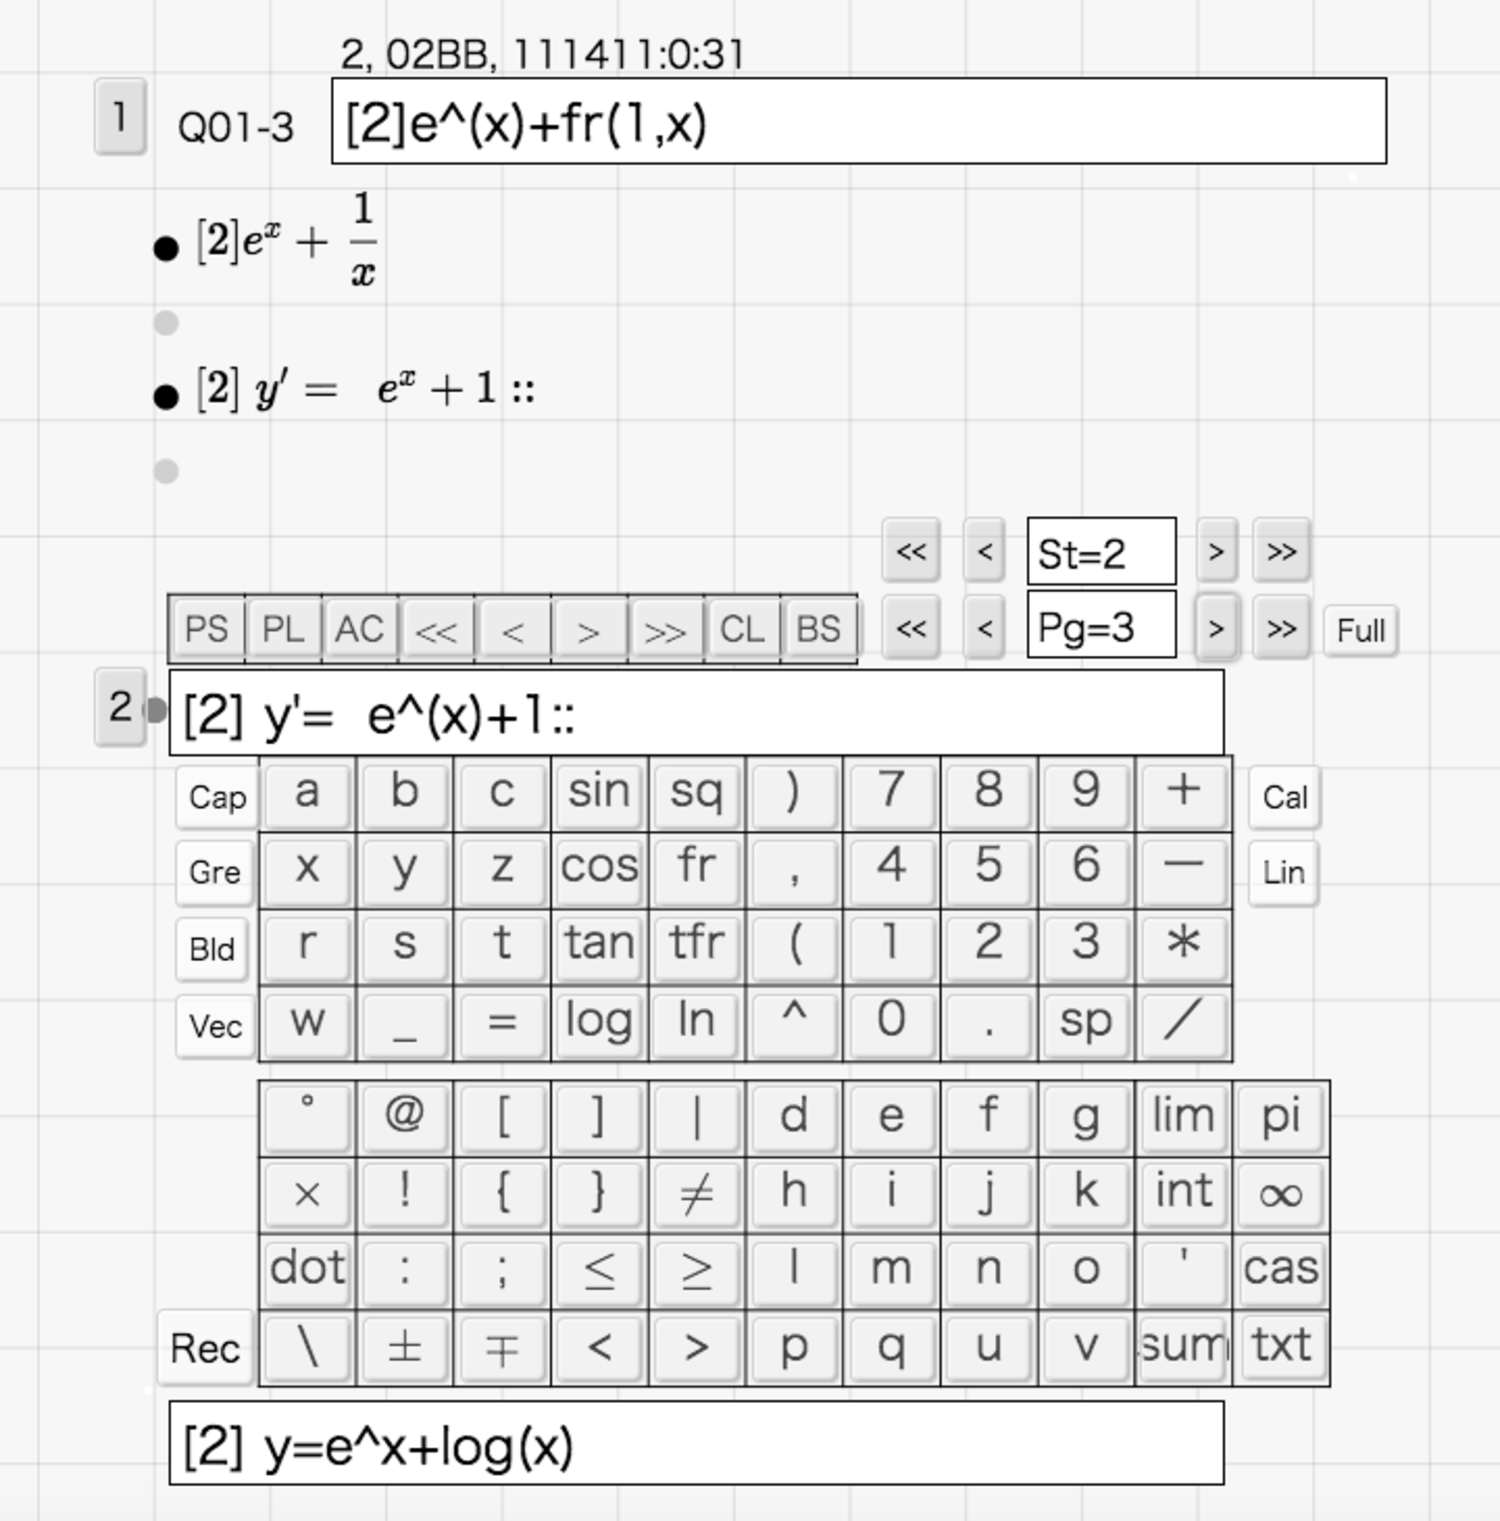
\includegraphics[bb=0.00 0.00 720.00 730.00,height=72mm]{fig/ketscore1bw.pdf}
\hspace{5mm}%
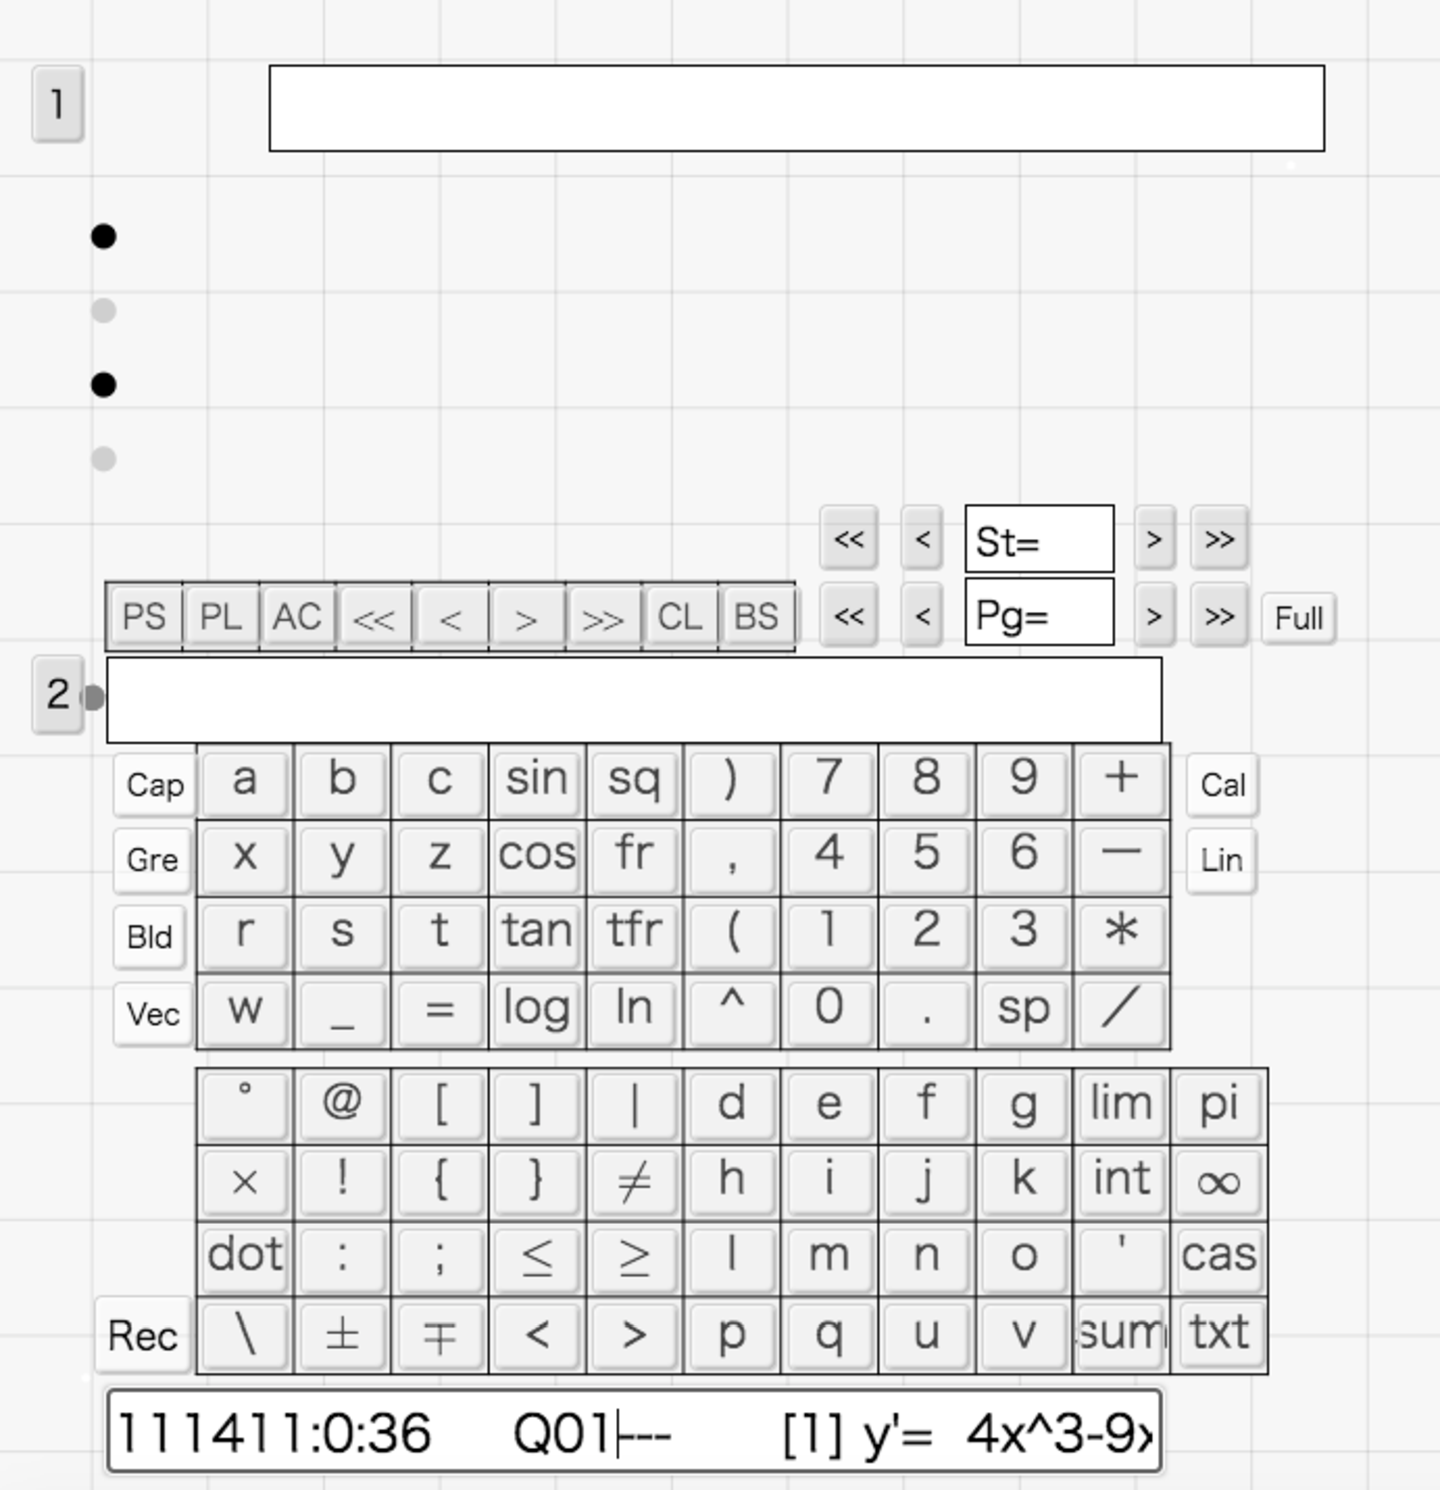
\includegraphics[bb=0.00 0.00 691.00 715.00,height=72mm]{fig/ketscore3bw.pdf}

\addtocounter{figure}{1}Fig.\thefigure\ \ ketscoreの画面\vspace{-1mm}
\end{center}

kettask以前は,解答をketmathに入力して確認してから送信するように指導していたが,スマホでは2つのアプリを同時に立ち上げて切り替えて実行することができないため,
KeTMathを使わずにそのまま数式を送信してくる学生が多かった.そのため,Maximaでの採点時にエラーが頻発して実用的とは到底いえなかった.kettaskを用いるようになってからは,問題を解くときに即時に\TeX 数式が確認できるようになったので,入力ミスは激減して,Maximaでの採点の実用性が増している.

\section{toolketmathによる結果の返却と分析}

採点が終わって4scoresheet.txtが確定したとき,toolketmath.cdyを立ち上げて
「成績票の作成」と「個別結合データ」を順に押すと,学生ごと問題ファイルごとの個別成績票st01task1130-01.txt(st01は学生番号,-01は問題ファイル番号)と学生について1つのテキストファイルにした学生ごとの成績票1130totalst01.txtがdata内のサブフォルダに作成される.\vspace{-0.5zw}

\begin{verbatim}
  1130-01の結果
  2 02BB 1130 11:0:31
  Q01 次の関数を微分せよ.
  [1]  y=x^4-3x^3+x^2+2x-3
   正解 4x^3-9x^2+2x+2
   答え 4x^3-6x^2+2x+3
   得点 0
  [2]  y=e^x+log(x)
   正解 e^(x)+fr(1,x)
   答え e^(x)+1
   得点 0
     ・・・・・
\end{verbatim}
\vspace{-0.5zw}

成績票totalstを送るために,著者らはDropboxのリンクを利用している\footnote{著者らは.他の方法に詳しくなく,Dropboxでのやり取りに習熟していることによる.}
具体的には\vspace{-1mm}

\begin{enumerate}
\item toolketmathのScriptにユーザーフォルダのパスDirdistを記述しておく.\\
\hspace*{2zw}\verb|Dirdist=Gethome()+"/Dropbox/”+成績フォルダ名;|\footnote{Gethome()は\ketcindy の関数でユーザホームのパスを返す}\vspace{-2mm}
\item toolketmathの「結合データを複写」を押すと,Dirdist内の学生ごとの
サブフォルダ’(ない場合は新規に作成される)に結合成績票がコピーされる.
\item Dropboxで各フォルダのリンク先を取得して,学生に個別に知らせる.
以後のデータも同じフォルダにコピーされるので,リンク先は1度だけ伝えておけばよい.\vspace{-2mm}
\item 学生はDropboxに登録していなくても3のリンク先にアクセスすることができる.
\end{enumerate}\vspace{-1mm}

toolketmathの「クラス結果作成」のボタンを押すと,次のようなcsvファイルができる.
\begin{center}
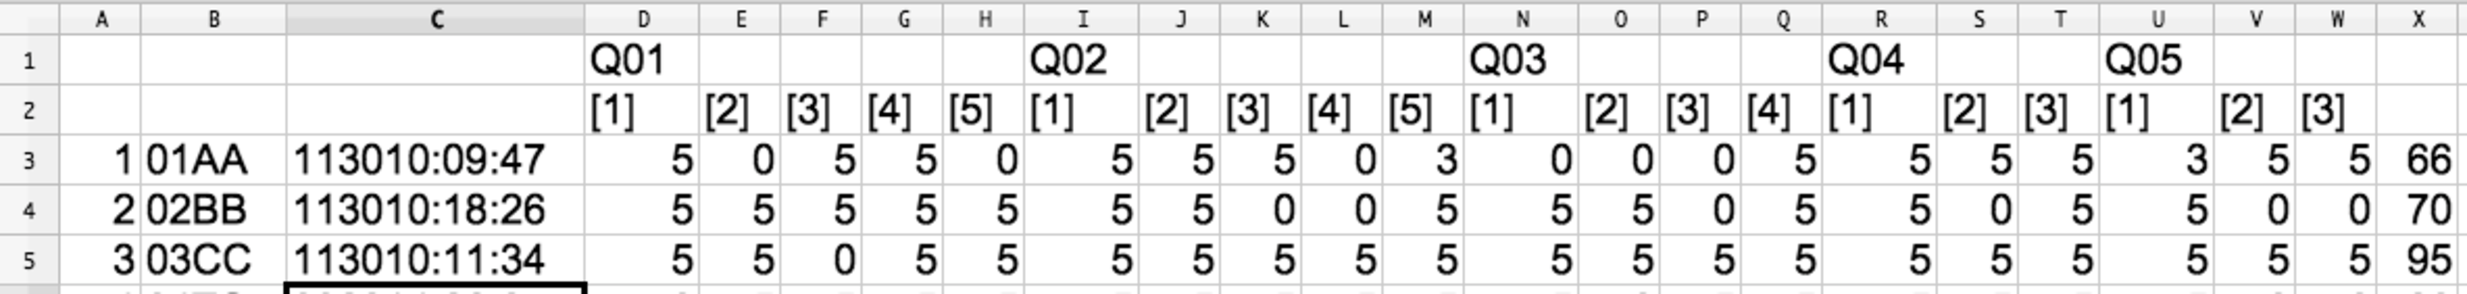
\includegraphics[bb=0.00 0.00 1184.00 141.00,width=140mm]{fig/csvbw.pdf}
\end{center}

\newpage

\noindent
{\bf 謝辞} 本研究はJSPS科研費22K02972の助成を受けている.

\begin{thebibliography}{00}

\bibitem{Cinderella1} Gebart J, Kortenkamp U., The Interactive Geometry Software Cinderella, Springer, 1999.

\bibitem{Cinderella2} Gebart J, Kortenkamp U., The Cinderella.2 Manual, Springer, 2012.

\bibitem{cindyjs} Gagern M., Kortenkamp U., Gebart J., Strobel M., CindyJS-- Mathematical Vsisualization on Modern Devices--, ICMS 2016, LNCS \textbf{9725}, 319--334, Springer, 2016.


\bibitem{rimstaka2178}
高遠節夫, 濱口直樹, Web利用の理数教育に役立つ数式送受システムの開発, 京都大学数理解析研究所講究録2178, 2021

\bibitem{rimstaka2208}
高遠節夫, 濱口直樹, 北本卓也, テキストをベースとしたLMSの利用とHTML教材の作成, 京都大学数理解析研究所講究録2208, 2022

\bibitem{rimstaka2208}
高遠節夫, 濱口直樹, 北本卓也, 1 次元表現ルールに基づいた数式の送受と授業実践, 城西大学数学科数学教育紀要(投稿中)

\end{thebibliography}


\end{document}

